% !TEX TS-program = pdflatex
% !TEX encoding = UTF-8 Unicode
\documentclass[12pt]{report}
\usepackage[utf8]{inputenc} % set input encoding (not needed with XeLaTeX)

\usepackage{geometry} % to change the page dimensions
\geometry{a4paper} % or letterpaper (US) or a5paper or....
\geometry{margin=2cm} % for example, change the margins to 2 inches all round

% Packages
\usepackage{pdflscape}
\usepackage{graphicx} % support the \includegraphics command and options
\usepackage[parfill]{parskip} % Activate to begin paragraphs with an empty line rather than an indent
\usepackage{booktabs} % for much better looking tables
%\usepackage{array} % for better arrays (eg matrices) in maths
%\usepackage{paralist} % very flexible & customisable lists (eg. enumerate/itemize, etc.)
%\usepackage{verbatim} % adds environment for commenting out blocks of text & for better verbatim
\usepackage{subfig} % make it possible to include more than one captioned figure/table in a single float
\usepackage{url}

% Headers and Footers
\usepackage{fancyhdr} % This should be set AFTER setting up the page geometry
\pagestyle{fancy} % options: empty , plain , fancy
\renewcommand{\headrulewidth}{0pt} % customise the layout of headers and footers
\lhead{Initial Plan}\chead{}\rhead{Iain Johnston}
\lfoot{}\cfoot{\thepage}\rfoot{}

% Section Title Appearance
\usepackage{titlesec}
\titleformat{\section}{\large\bfseries}{\thesection}{1em}{\hrule}

% ToC appearance
\usepackage[nottoc,notlof,notlot]{tocbibind} % Put the bibliography in the ToC
\usepackage[titles,subfigure]{tocloft} % Alter the style of the Table of Contents
\renewcommand{\cftsecfont}{\rmfamily\mdseries\upshape}
\renewcommand{\cftsecpagefont}{\rmfamily\mdseries\upshape} % No bold!


% The document content starts below

\title{\textit{Initial Plan}\\\textbf{Maximising entertainment value in the vote-reveal problem}\\ Final Year Project (CM3203) - 40 Credits}
\author{Author: Iain Johnston (1312579) \\ Supervisor: Richard Booth\\ Moderator: Xianfang Sun}
\date{} % Activate to display a given date or no date (if empty),  otherwise the current date is printed

\begin{document}
\maketitle

\tableofcontents %  place a table of contents after the title
\clearpage % clear the page after the table of contents

%\addcontentsline{toc}{section}{Section z} % how to add an entry to the table of contents that is un-numbered
%\section*{Second Section} % an un-numbered section in the document
%\subsection{A subsection} % an example subsection

  
\section*{Project Description}
\addcontentsline{toc}{section}{Project Description}
In many elections or competitions, a set of voters will rank a set of candidates from best to worst, or will give scores to some of the candidates, with the winner then being the candidate that gets the highest total number of points. When it comes to revealing the result after all votes have been cast, some competitions proceed by having a roll-call of all the voters in which each announces their own scores. This is often done for entertainment purposes such as in the Eurovision Song Contest.\cite{ref:EurovisionVoting}

The concept of entertainment, especially with respect to competition, is heavily subjective subject and as such is hard to quantify in simple terms. There are intuitive constituent parts to an \textit{entertaining} competition (like Eurovision) such as, if the winner is known early or late, and how many teams are in the running to win. A large constituent part of this project will be to convert these intuitive ideas into mathematical values that can then be maximised by some optimisation algorithm. 

The two main questions that this project will aim to answer are:

\begin{enumerate}
\item How can we define the concept of ''entertainment'' in the context of an optimisation problem, and hence try to maximise it.
\item  In which order should the votes be revealed in order to maximise that entertainment value?
\end{enumerate}

To try and answer these questions I will be using the Eurovision Song Contest as my example as it has many datasets, having been running annually since 1956. Furthermore voting rules have gone through changes over the years as more countries joined and as it grew in popularity, giving the project a natural comparison tools throughout. 

Most recently since the 2016 running of the contest, the jury votes and the public votes are given separately instead of being combined into one score. This change was apparently made "...to make a better television show as well as a more exciting competition"\cite{ref:NewVotingQuote}. This change can form part of the final report on how the algorithm and entertainment function has performed compared to the real contest.

This change shows that the motivation behind this project, to maximise entertainment when revealing the votes, is a current problem and there have been attempts to try and solve this problem already.

\section*{Project Aims and Objectives}
\addcontentsline{toc}{section}{Project Aims and Objectives}
There are three main aims that this project will attempt to tackle, as well as some smaller objectives. These aims are described below.

\subsection*{1. Entertainment Value}
\addcontentsline{toc}{subsection}{Entertainment Value}
The most important of the aims of this project is to come up with some function(s) to measure the "entertainment value" of a given roll-call. 

This is a way of mapping a roll-call ordering to a single entertainment value. This would be a mathematical function that given an ordering of members in the competition, should return a value that gives an estimation of how entertaining that ordering is. As entertainment is a heavily subjective topic, this part of the project will have to have justification of why I think a function correctly describes an entertaining roll-call. This justification will likely be in the form of comparisons to real-world tournaments or competitions in which the intuitive theory behind a function has been seen to be entertaining. 

To find a good function for this entertainment value I will start with an intuitive idea and then define a mathematical representation of that idea. Then I will use that as a cost function in the optimisation algorithm and analyse the results to see if it is indeed an entertaining roll-call.

It may be necessary to define multiple functions however that depends entirely on how well the first chosen function performs and if it can provide at least a near optimal solution to the problem.

A simple diagram explaining the methodology of getting an entertainment value is shown below:

\begin{figure}[h]
\label{entertainmentFunctionDiagram}
\caption{Entertainment Function Diagram}
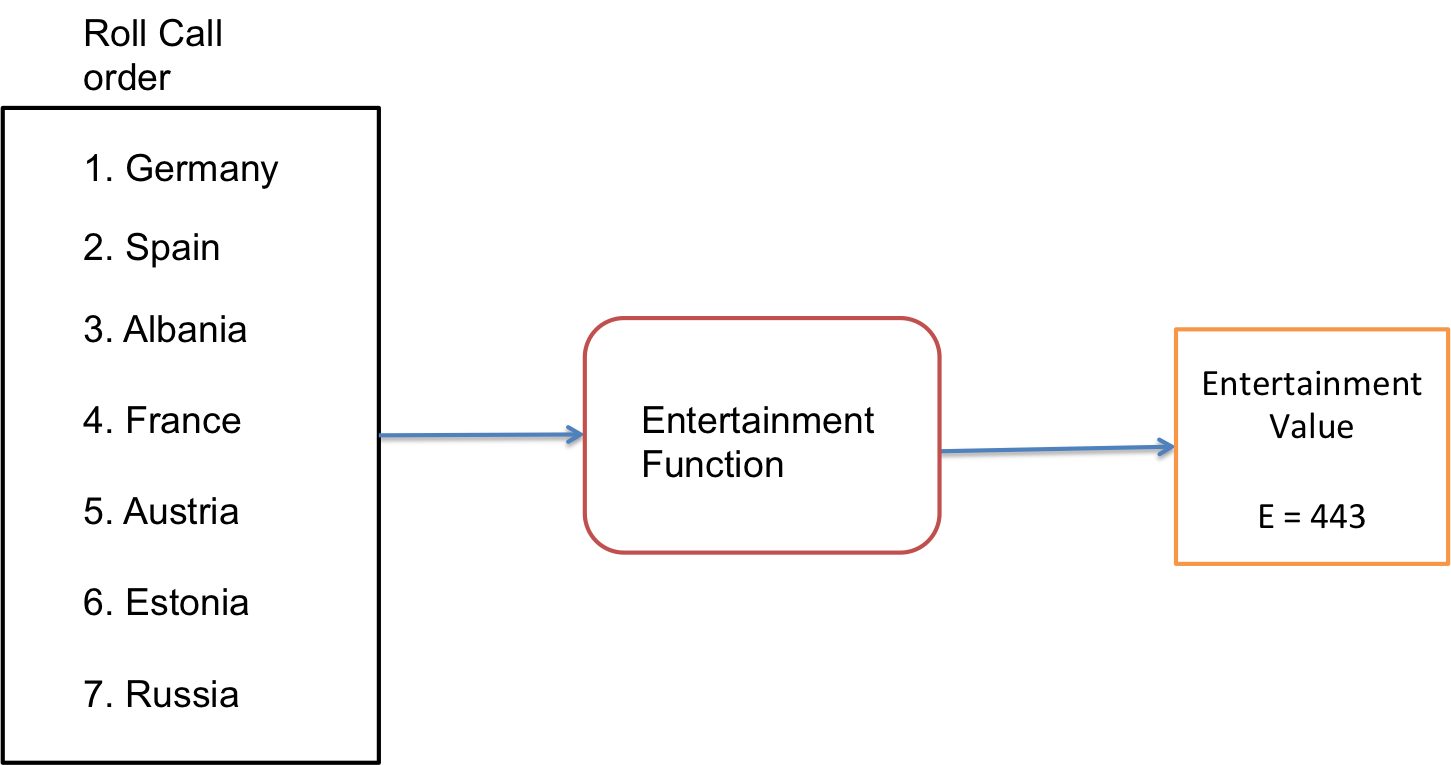
\includegraphics[scale=0.75]{EntertainmentFunctionDiagram.png}
\end{figure}

\subsection*{2. Optimisation Algorithm}
\addcontentsline{toc}{subsection}{Optimisation Algorithm}
Another of the main aims is the solve the optimisation problem of finding a roll-call that maximises an entertainment function.

Solving the optimisation problem will involve choosing a viable algorithm or algorithms that can solve the optimisation problem. Then it will involve implementing those algorithms with added problem specific code and additions to allow it to optimise the given cost function.

To start with I will try and keep the algorithm simple and create a greedy algorithm\cite{ref:GreedyAlgorithms1}\cite{ref:GreedyAlgorithms2} and if the problem space is sufficiently simple then this may be good enough to find an optimal solution. For this objective it will be necessary to design and write the algorithm itself with respect to the problem we are trying to solve as well as with respect to space and time complexity.

In this problem the greedy algorithm will be choosing the solution that maximises the entertainment value produced by the entertainment function at every step.

\subsection*{3. Visualisation of Problem and Solution}
\addcontentsline{toc}{subsection}{Visualisation of Problem and Solution}
An important part of the project will be being able to show how the algorithm computes its solution and how that solution compares to the real-world. To meet this aim I will create a simple web application that visualises the algorithm running and can compare it the actual running of the Eurovision contest.

This application will have a way of stepping through the voting reveal stages showing both my implementations ordering, current scores and teams and the actual contest side by side. The hope is that this will add another way to justify why the entertainment function and algorithm are correct in being entertaining and giving others a chance to judge for themselves.

\section*{Ethics}
\addcontentsline{toc}{section}{Ethics}
I have not identified any ethical issues\cite{ref:Ethics} with this project as there will no personal data used and the Eurovision Song Contest data I will use is publicly and lawfully available.

\section*{Work Plan}
\addcontentsline{toc}{section}{Work Plan}
The overall plan for the project is split into three parts, designing and implementing entertainment functions, designing and implementing an optimisation algorithm and visualising the final results. These three parts have been further subdivided in the time plan and Gantt chart to give a more granular view of what each week of the project will entail. 

Although the overall plan will very likely stay the same throughout, the time scales may change during the project. In the time plan and the Gantt chart the task are marked with a letter denoting the main aim or objective of which they are a necessary part. \textbf{E} for work on the entertainment value, \textbf{A} for the optimisation algorithm and \textbf{V} for the visualisation. Some task are a part of more than one of these.

\subsection*{Deliverables}
\addcontentsline{toc}{subsection}{Deliverables}
The deliverables for this project will be:
\begin{enumerate}
\item Final Report
\item Source code of the optimisation algorithm used
\item Datasets used to test algorithm
\item Visualisation of problem and solution
\end{enumerate}

\subsection*{Milestones}
\addcontentsline{toc}{subsection}{Milestones}
The main milestones for this project are: 

\begin{itemize}
\item the successful running of an algorithm against a dataset
\item a way of visualising the algorithms running and how the algorithm I have used compares to real-world examples
\end{itemize}
These milestones come in at Week 10 for having a running algorithm and Week 14 for having a visualisation.

To reach these milestones and the final deliverables described above, I plan to spend every week day working on the project between the hours of 09:00 and 17:00. Of course this does not include the time during which I have lectures or labs and furthermore one of the days every week must be kept free as I continue my part-time job from my placement year.

The time plan below is a rough way of showing the things that I will be working on during each given week. It is supported by a Gantt chart which is attached in the appendix. The Gantt chart will be updated every week by filling out the "actual start" and "actual duration" parts of each task. This will then provide evidence of the project work during the final report.

Week 1 begins on the 23rd January before giving in this Initial Plan. In this plan and in the attached Gantt chart I have continued my numbering of the weeks over the Easter break. This means that Week 15 in the plans corresponds to teaching week 12 and hence the deadline for the Final Report is the end of Week 15 in both plans.

\subsection*{Time Plan}
\addcontentsline{toc}{subsection}{Time Plan}

\textbf{Week 1 (23/01/17)}
\begin{itemize}
\item \textbf{V/E/A} - Write Initial Plan - \textit{Deadline: 30/01/17}
\end{itemize}

\textbf{Week 2 (30/01/17)}
\begin{itemize}
\item \textbf{E/A} - Research
\end{itemize}

\textbf{Week 3 (06/02/17)}
\begin{itemize}
\item \textbf{E} - Define entertainment functions
\end{itemize}

\textbf{Week 4 (13/02/17)}
\begin{itemize}
\item \textbf{First review meeting}
\item \textbf{A} - Write skeleton algorithm
\end{itemize}

\textbf{Week 5 (20/02/17)}
\begin{itemize}
\item \textbf{A} - Gather and prepare data for use
\end{itemize}

\textbf{Week 6 (27/02/17)}
\begin{itemize}
\item \textbf{A} - Write problem specific algorithm
\end{itemize}

\textbf{Week 7 (06/03/17)}
\begin{itemize}
\item \textbf{A} - Write problem specific algorithm
\end{itemize}

\textbf{Week 8 (13/03/17)}
\begin{itemize}
\item \textbf{A} - Write problem specific algorithm
\item \textbf{Second review meeting}
\end{itemize}

\textbf{Week 9 (20/03/17)}
\begin{itemize}
\item \textbf{A} - Write problem specific algorithm
\item \textbf{V} - Create visualisation of results
\end{itemize}

\textbf{Week 10 (27/03/17)}
\begin{itemize}
\item \textbf{V} - Create visualisation of results
\item \textbf{V/E/A} - Run experiments on datasets
\end{itemize}

\textbf{Week 11 (03/04/17)}
\begin{itemize}
\item \textbf{V} - Create visualisation of results
\item \textbf{V/E/A} - Analyse data from experiments
\end{itemize}

\textbf{Week 12 (10/04/17)}
\begin{itemize}
\item \textbf{V} - Create visualisation of results
\item \textbf{V/E/A} - Write final report
\end{itemize}

\textbf{Week 13 (17/04/17)}
\begin{itemize}
\item \textbf{V} - Create visualisation of results
\item \textbf{V/E/A} - Write final report
\end{itemize}

\textbf{Week 14 (24/04/17)}
\begin{itemize}
\item \textbf{V} - Create visualisation of results
\item \textbf{V/E/A} - Write final report
\end{itemize}

\textbf{Week 15 (01/05/17)}
\begin{itemize}
\item \textbf{V/E/A} - Finish and hand-in final report - \textit{Deadline: 05/05/17}
\end{itemize}

\clearpage
\renewcommand{\bibsection}{\section*{References}}
\addcontentsline{toc}{section}{References}
\bibliography{/Users/johnsi63/Desktop/InitialPlan/References/initialPlanBib}{}
\bibliographystyle{ieeetr}


\clearpage
\addcontentsline{toc}{section}{Appendix}
\begin{landscape} 
\section*{Appendix}
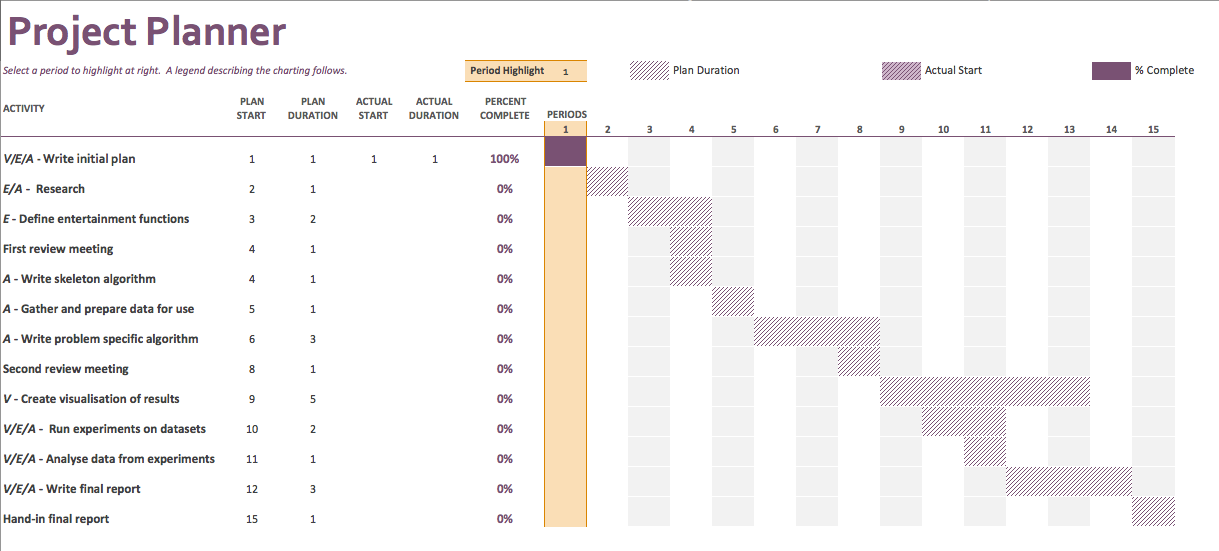
\includegraphics[height=14.5cm, width=\linewidth]{InitialPlanGanttChart.png}
\end{landscape}

\end{document}
